\section{Analysis of Track Reconstruction with AI}

After implementing the track identification service in the CLAS12 reconstruction software, the outputs
from the conventional tracking algorithm and AI-assisted tracking algorithm were analyzed
event by event to assess the improvements of tracking. 
 
 \subsection{Particle Reconstruction efficiency}
 
 The Neural Network for track classification was trained on experimental data after it was processed with conventional tracking. Tracks that had ``good'' fit quality and were tracked back to the target location were used as training samples for both 
 the MLP classifier and Auto-Encoder corruption-recovery network. 
 Performance was assessed on data recorded at CLAS12 production settings, specifically with 45 nA electron beam impinging on a 5 cm-long hydrogen target for an instantaneous luminosity close to $10^{35} cm^{-2} s^{-1}$.
% For more detailed analysis of tracking reconstruction performance with and without assistance from artificial intelligence we processed one run at nominal luminosity (45 nA) to compare performances.
 
 %The efficiency of track reconstruction was obtained for separate track topologies (6 super-layer and 5 super-layer).
 \begin{figure}[!ht]
\begin{center}
% 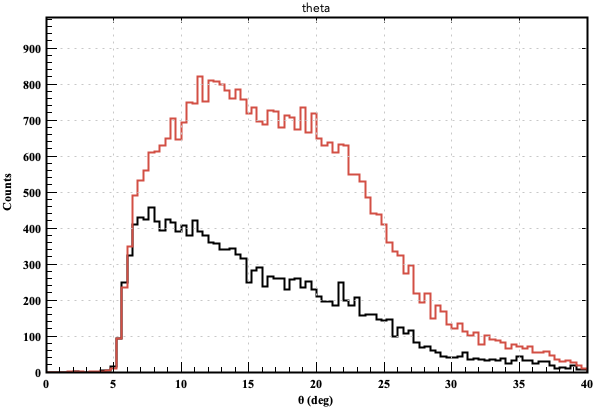
\includegraphics[width=2.0in]{images/pos_theta_5SL.png}
  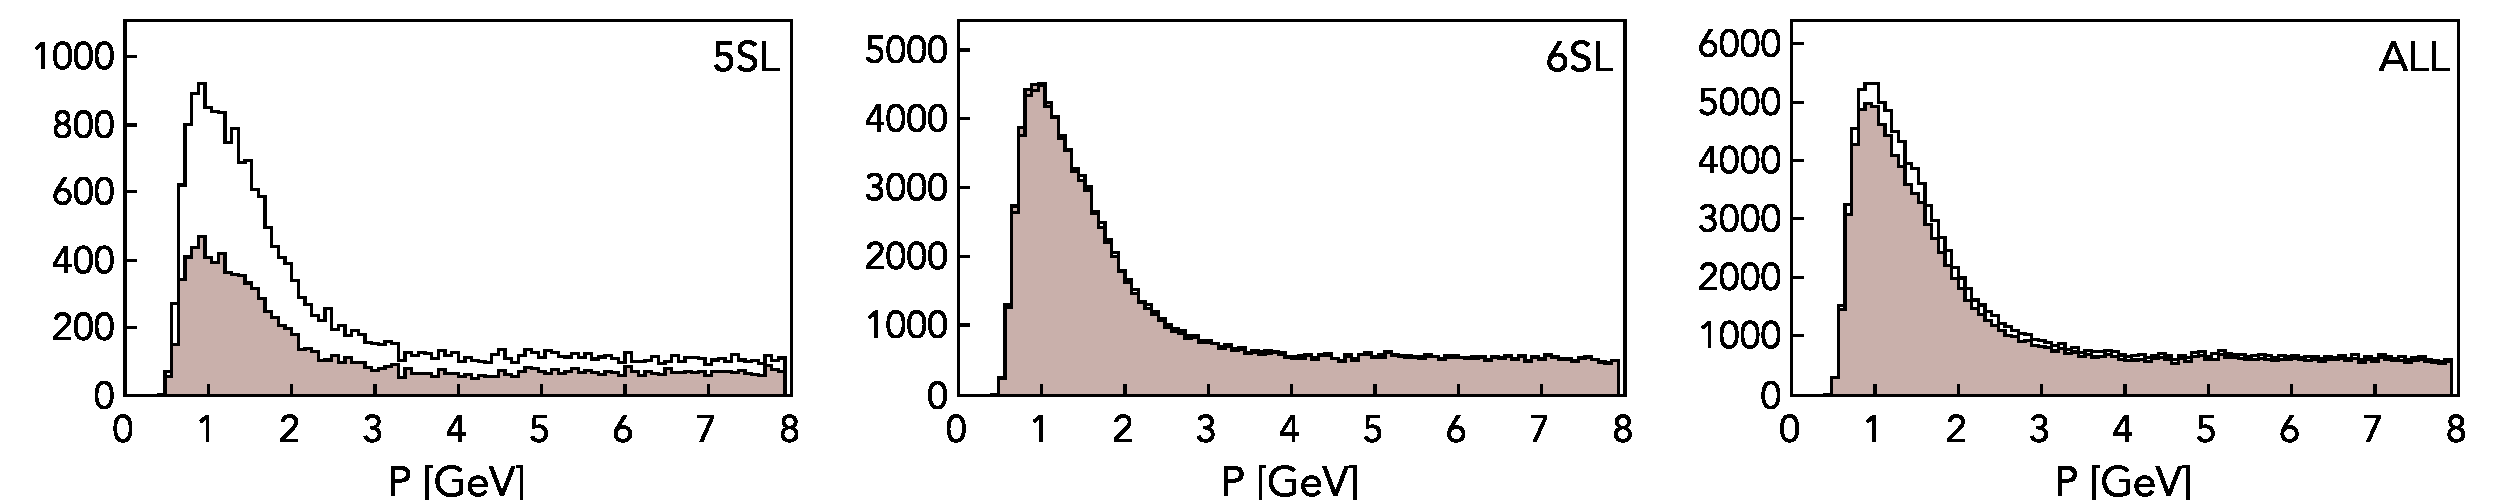
\includegraphics[width=6.5in]{images/figure_p.pdf}
  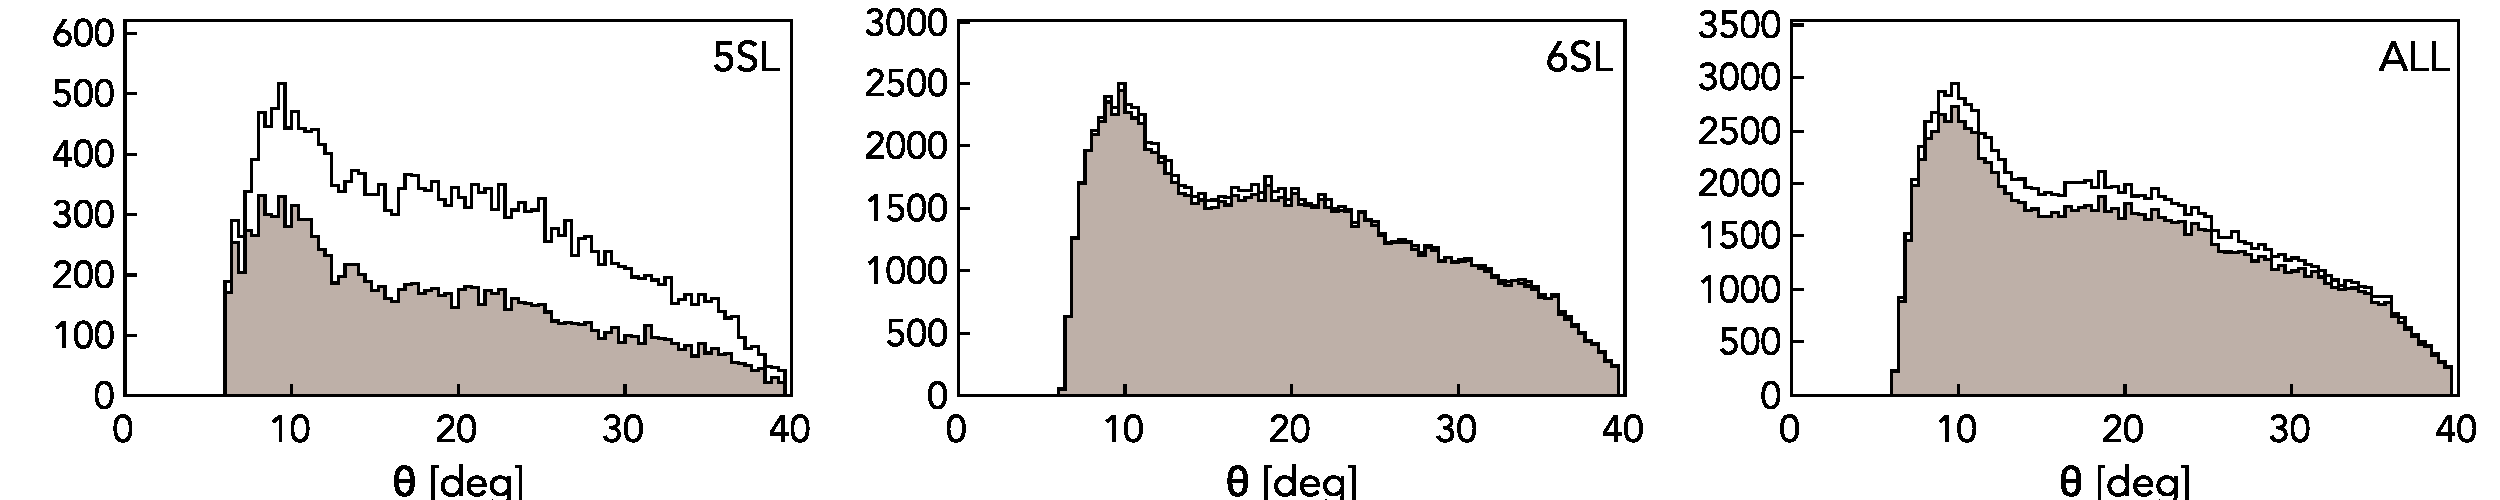
\includegraphics[width=6.5in]{images/figure_theta.pdf}
    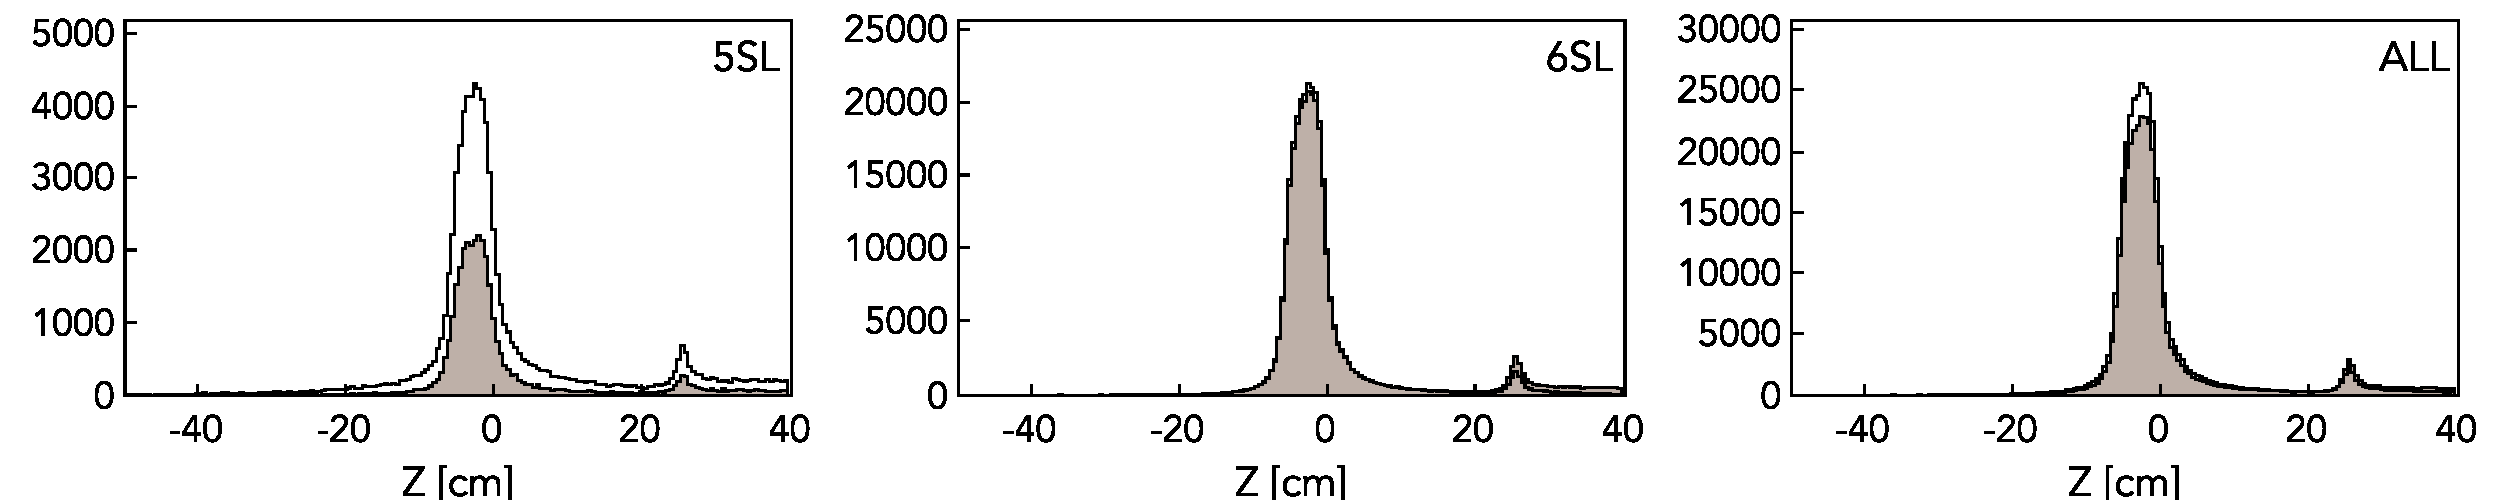
\includegraphics[width=6.5in]{images/figure_vz.pdf}
\caption { Comparison of number of tracks reconstructed with the conventional algorithm (filled histograms) vs AI-assisted tracking code (open black outline histograms) as a function of momentum, polar angle and particle interaction vertex. The comparison is shown for 5 super-layer, 6 super-layer tracks (left two columns), and the total number (right column).}
 \label{track:efficiency}
 \end{center}
\end{figure}

The results are shown in Figure~\ref{track:efficiency}, where the dependence of number of ``good'' reconstructed negatively charged 
 tracks are shown as a function of particle momentum (top row), polar angle in laboratory frame (bottom row) and interaction
 vertex (middle row). The reconstructed distributions from conventional tracking are plotted with filled histograms and the
 tracks reconstructed using assistance from AI are plotted with solid lines. As can be seen from the figure, there is a large gain 
 in the number of reconstructed tracks with the 5 super-layer configuration compared to full 6 super-layer tracks. Typically for nominal 
 45 nA experimental data increase in track efficiency averages about $3\%-6\%$ for 6-sperlayer tracks and to $70-120\%$ for 5-superlayer tracks 
 %, while for 5 super-layer
 %tracks the increase is in the order of $70\%-120\%$. 
 In conventional data reconstruction, tracks that are identified with 5 super-layers usually comprise about $10\%$ of all reconstructed tracks, 
 and a significant increase in identification of such tracks leads to overall tracking efficiency increase of $10\%-15\%$. 
 
 \begin{table}[!h]
 \begin{center}
 \begin{tabular}{|l|c|c|c|c|}
 \hline
 Track Configuration & Conventional & AI Assisted & Gain & Relative \\
 \hline
 \hline
 6 Super-Layer & 242,145 & 256,175 & 14030 & 1.0579 \\
 5 Super-Layer & 24,155 & 52,839 & 28684 & 2.1875 \\
 All & 267,339 & 309,058 & 51719 & 1.1561 \\
 \hline
 \end{tabular}
 \end{center}
 \caption{Summary of reconstructed tracks and gain with assistance from Artificial Intelligence.}
 \label{tbl:summary}
 \end{table}
 
The comparison of 5 and 6-segment track statistics and their relative gain is summarized in Table~\ref{tbl:summary}.
As can be seen from the table, the gain in 6-segment tracks is about $8\%$ but with significant gain in 5 super-layer tracks 
the overall gain in reconstructed tracks elevates to $>15\%$. These results are intuitive since the number of track candidates composed of 5
super-layers, assuming a uniform number of clusters in the six super-layers, is significantly higher than 6 super-layer track candidates, and 
in our tests AI performs better in choosing the right combination with increasing combinatorics.
%the number of
%with the same number of clusters in each super-layer are 
 
\subsection{Luminosity Dependence}
As discussed in the previous section, AI is more efficient than the conventional track-finding algorithm in identify good candidates from a large pool.
One would expect that, if the number of combinations decreases, the efficiency of the conventional track selection should approach the efficiency of 
AI-assisted track identification. Similarly, when the number of combinations increases the gain of AI over the conventional algorithm should
increase. Based on this we expect AI to perform better in higher luminosity, higher background settings. To evaluate the AI-assisted tracking efficiency 
dependence on background we analyzed several different runs that were taken in different conditions (i.e. beam current) ranging from $5~nA$ to 
$70~nA$. To determine the tracking efficiency we first calculated the number of electrons ($N_e$) detected in the data sample analyzed (typically one run,
or $2h$ of data taking) and then the number of positive and negative hadrons that were detected with the electron inclusively ($N_{h^+e}$ and $N_{h^-e}$ respectively).

Then the efficiency for the data set was calculated as:

\begin{equation}
L_t^+ = \frac{N_{h^+e}}{N_e} , L_t^- = \frac{N_{h^-e}}{N_e} 
\end{equation}

where $L_t^+$ is the efficiency of positive particles and $L_t^-$ is the efficiency of negatively charged particles respectively. 
In order to estimate the charged particle reconstruction efficiency as a function of the beam current, the multiplicity, $L_t^{+/-}$, is fitted with a linear function:
\begin{equation}
L_t^{+/-} = a + b\times I 
\end{equation}

Here $a$ and $c$ are the fit parameters and $I$ is the beam current. Then it was assumed that the reconstruction efficiency, $E=1$ at $I=0$ nA:

\begin{equation}
E^{+/-} = 1 + c \times I 
\end{equation}

with $c=\frac{b}{a}$. The slope parameter $c$ represents the variation of the reconstruction inefficiency per $nA$~\cite{Stepanyan:2020bg}.
%The all points were 
%fitted with linear function $L=a+bx$, where $a$ is the intercept 
 
 \begin{figure}[!ht]
\begin{center}
 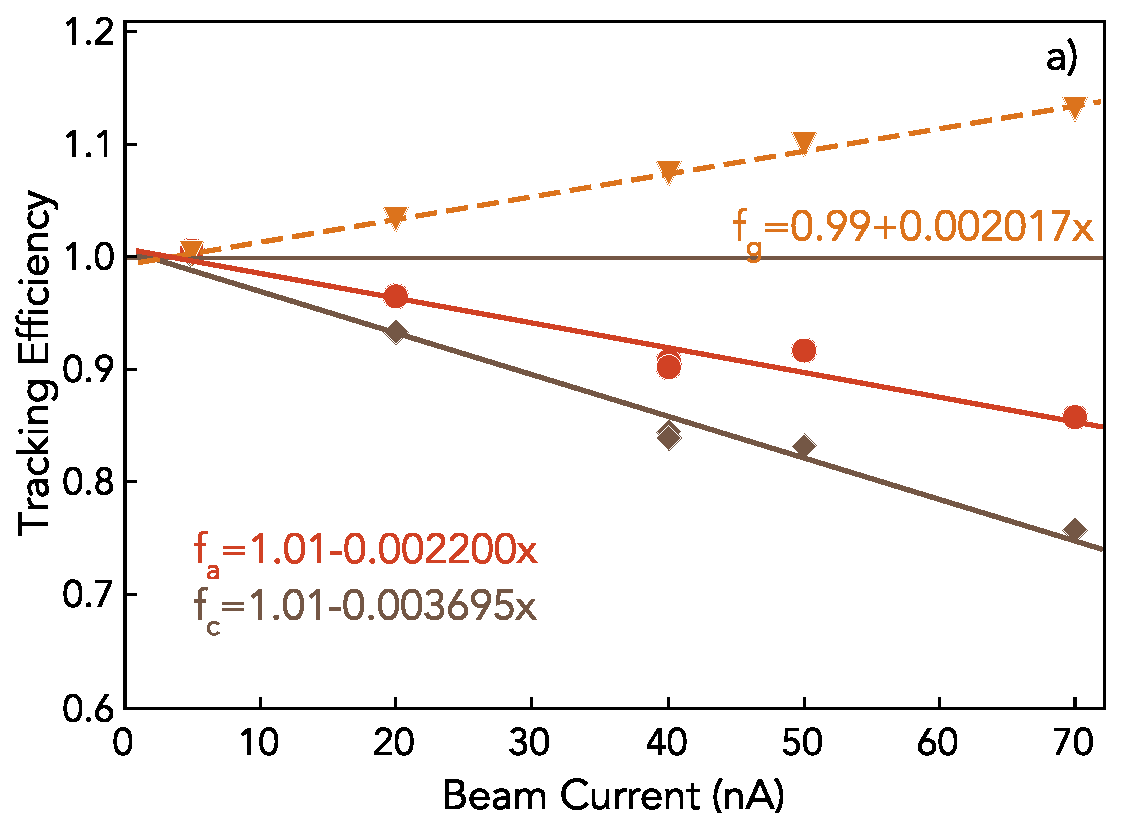
\includegraphics[width=3.0in]{images/figure_lscan_pos.pdf}
 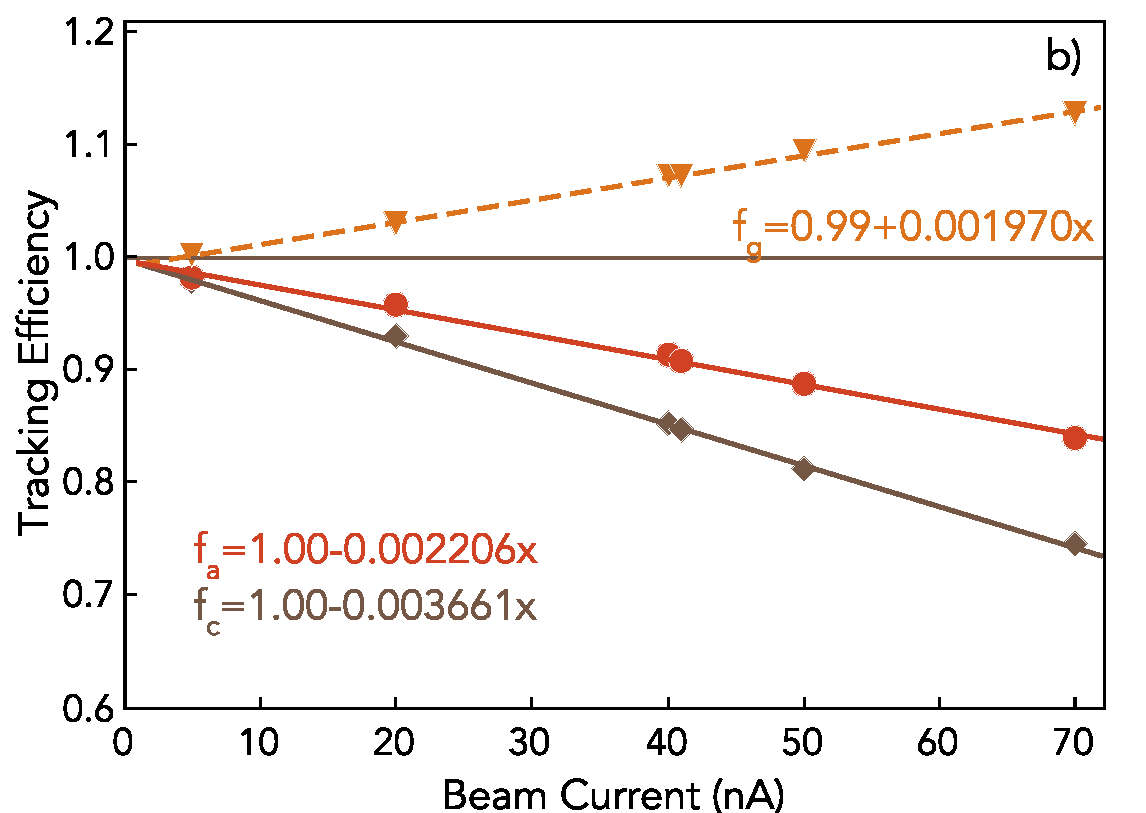
\includegraphics[width=3.0in]{images/figure_lscan_neg.pdf}
\caption {Tracking efficiency for positively and negatively charged particles as a function of beam current (luminosity).  Conventional algorithm 
track reconstruction efficiency (diamonds) is compared to AI-assisted track reconstruction efficiency (circles). }
 \label{lumi:scan}
 \end{center}
\end{figure}

The comparison of tracking efficiency as a function of beam current (luminosity) can be seen in Figure~\ref{lumi:scan} where $E^{+/-}$ are shown for positively and negatively charged particles separately. AI-assisted tracking performs significantly better for any given luminosity (beam current) and the decrease of efficiency is much slower as a function of luminosity, $0.22\%$ per nA versus $0.40\%$ per nA for conventional tracking. This is expected and consistent with the assumption that with increased combinatorial background (increased number of track candidates to consider), AI performs better in choosing the best track candidate. We established that AI-assisted
tracking leads to more tracks reconstructed for any given beam current setting. The next thing to check is what is the impact of increased track reconstruction efficiency on physics analysis.
% and if there is increase in physics outcome for the CLAS12 experimental setup.

\subsection{Physics Impact}

To measure the implications of track reconstruction efficiency improvements on physics analysis, we considered 
two event topologies with two and three particles in the final state, respectively. The data for analysis were 
taken with $10.6~GeV$ electron beam incident on $5~cm$ liquid hydrogen target, with a beam current of $45~nA$
(typical for CLAS12 experimental running). We selected events where an electron was detected in the forward detector, and 
then isolated events where there was an additional positively charged pion ($\pi^+$) along with an electron and no other 
charged particle. The second topology required two pions along with the electron, one positively charged and one 
negatively charged. The two chosen topologies are denoted by $H(e,e'\pi^+X)$ and $H(e,e'\pi^+\pi^-X)$. In both cases 
there is a visible peak of a missing nuclean that we can use to measure the impact of efficiency on physics outcome. 

 \begin{figure}[!ht]
\begin{center}
 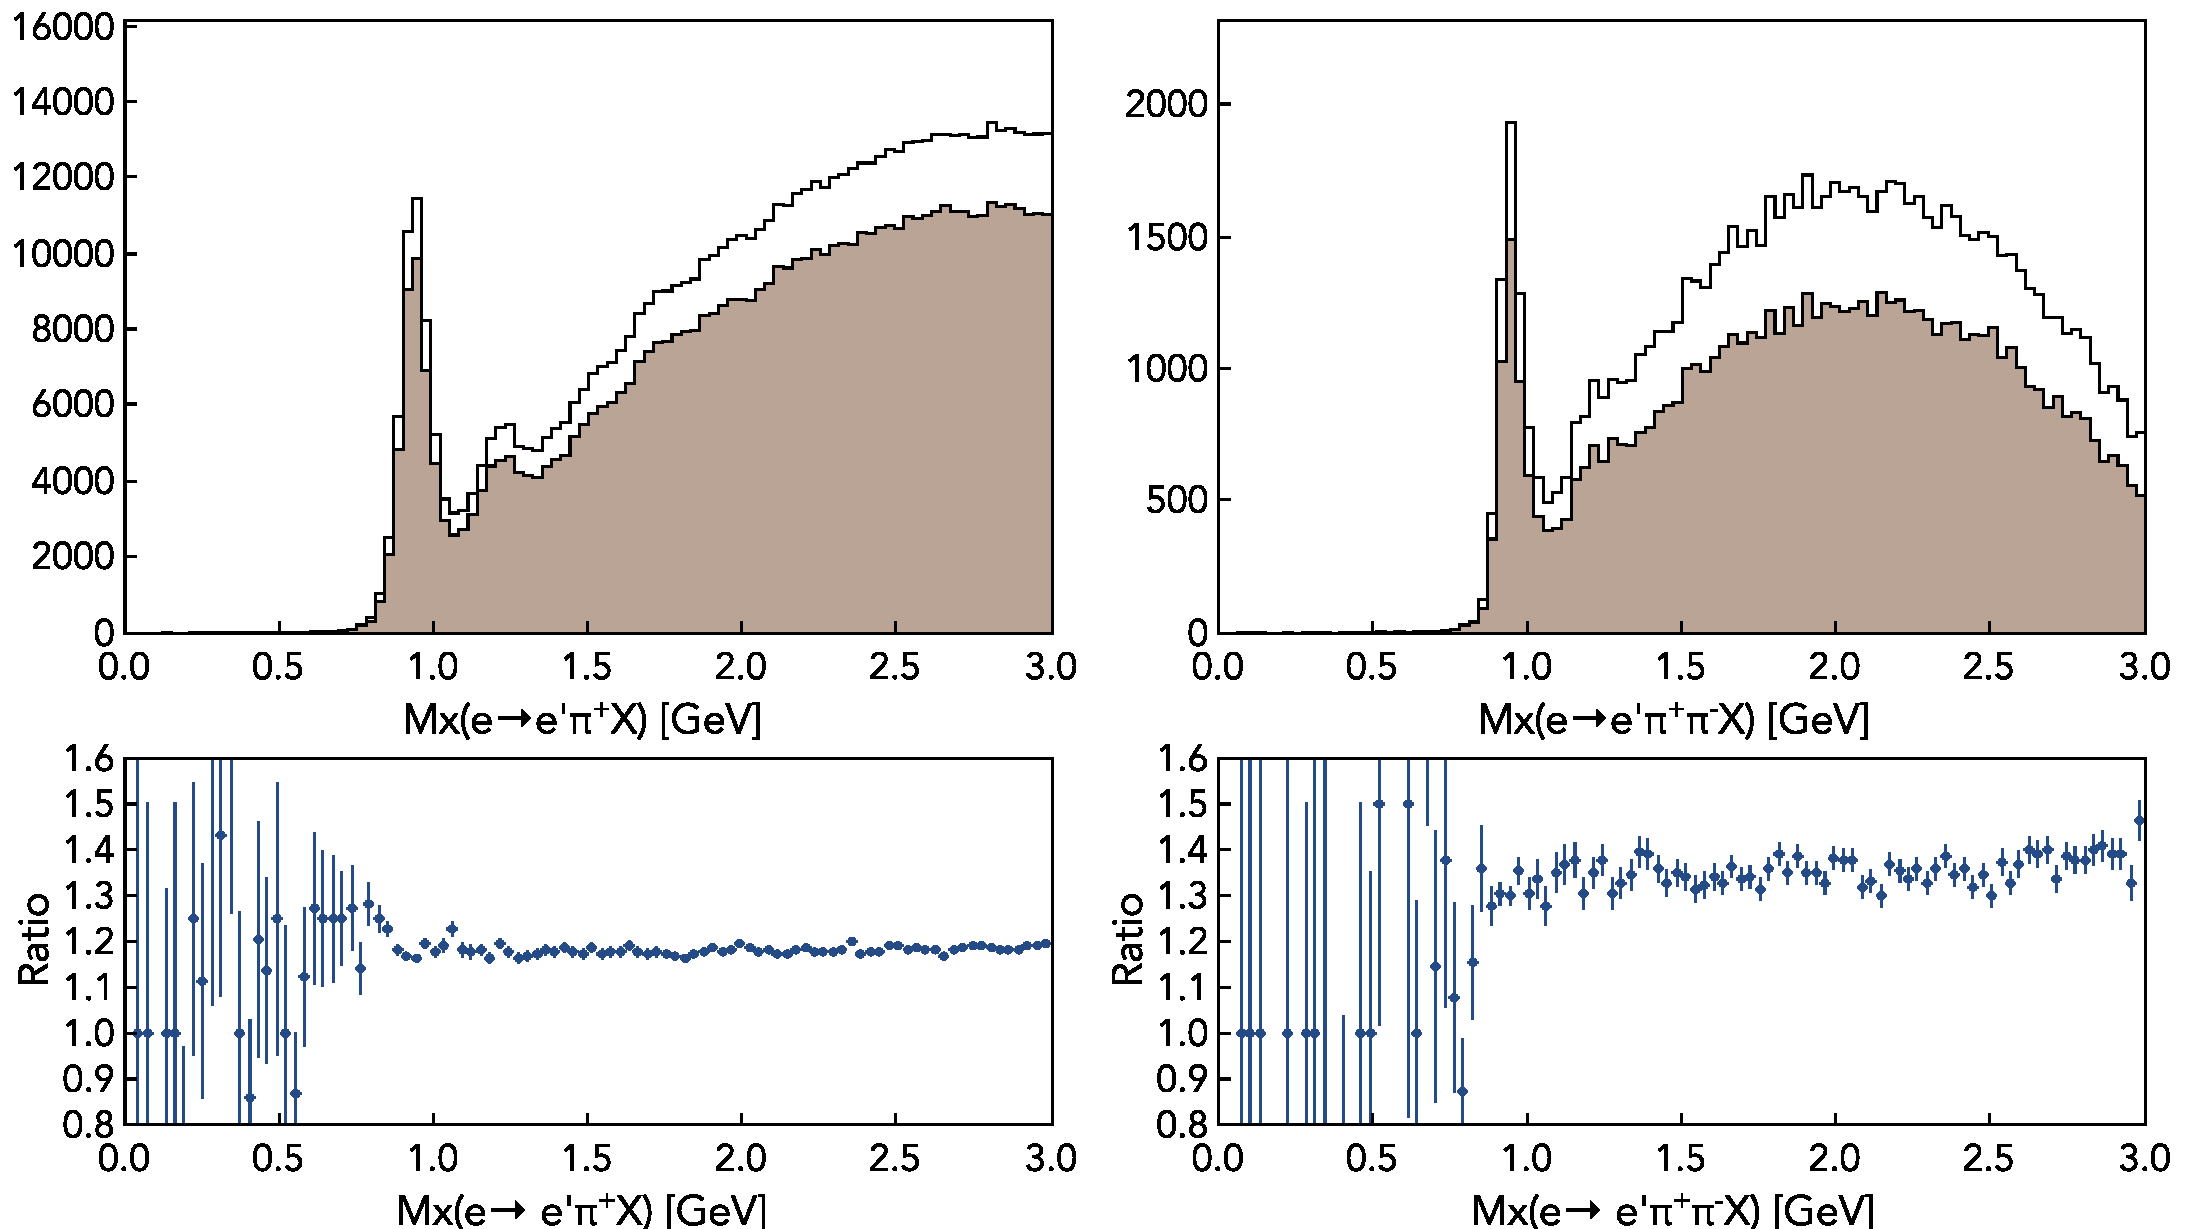
\includegraphics[width=6.0in]{images/physics_scan.pdf}
\caption {Reconstructed missing mass distribution for $H(e,e'\pi^+X)$ and $H(e,e'\pi^+\pi^-X)$ reactions (top row) using the conventional track reconstruction algorithm (filled histogram) and  AI-assisted track reconstruction (black line histogram). The ratios of the two histograms are shown on the bottom row. }
 \label{physics:outcome}
 \end{center}
\end{figure}

The distributions of missing mass for both final state topologies are shown on Figure~\ref{physics:outcome}, where the plots 
on the top row are missing mass of $H(e,e'\pi^-X)$ and $H(e,e'\pi^+\pi^-X)$, where the filled histogram is calculated from 
particles reconstructed by the conventional tracking algorithm, and the histogram with black outline are the same distributions 
calculated from particles that were reconstructed using suggestion from Artificial Intelligence. As can be seen from the figure, 
there is significant increase in the number of events in the region of the nucleon peak for AI assisted
tracking. The ratios of the two histograms (AI-assisted divided by conventional) can be seen on the bottom row of 
Figure~\ref{physics:outcome}. As can be seen from the figure the increase in statistics is uniform over the whole range of the 
missing mass indicating no systematic abnormalities for AI-assisted tracking. The ratio also indicates that there is an increase 
for the number of events of about $15\%$ for $H(e,e'\pi^+X)$ final state and $30-35\%$ for the $H(e,e'\pi^+\pi^-X)$
final state. Further studies show that improvements in statistics are larger for higher luminosity (incident beam current), which is consistent with our studies of increased efficiency of single particle reconstruction.
%Further studies show that increase in statistics for different final states increase with increase of beam current (luminosity) 
%which is consistent with our studies of increased efficiency of single particle reconstruction. 


\section{Summary}

In this paper we present results of the analysis of experimental data from the CLAS12 detector obtained with assistance of Artificial Intelligence
to identify tracks from the hits in drift chambers. This work is based on two neural networks developed to classify track candidates from
given cluster combinations \cite{Gavalian:2020oxg} and to identify missing cluster positions in tracks that do not have complete 6 cluster configuration \cite{Gavalian:2020xmc}. After implementing these networks into the CLAS12 reconstruction workflow, AI was able to identify ``good'' track candidates 
and pass them to the tracking code to be analyzed in parallel to conventional algorithms that chooses ``good'' track candidates iteratively considering all possible combinations. 
Our studies showed that AI-assisted tracking performs better than conventional track identification algorithm, and leads to track reconstruction efficiency increase of $10-15\%$ for nominal experimental running conditions (beam current 45 nA). The AI also performs better with increasing background (i.e. with increased incident beam current) and improves the efficiency loss from $0.44\%$ per nA to $0.24\%$ per nA.
This increased track reconstruction (identification) efficiency directly impacts the outcome of physics analysis, where it leads to an increase of statistics of 
$15\%-35\%$, depending on how many particles are detected in the final state. This has significant implication on  the choice of experimental running conditions since with increased efficiency the required statistical significance can be reached in a shorter time by running at higher beam current (luminosity). Already collected experimental data can be re-processed with the AI-assisted tracking
code which can increase the statistics available for physics analysis up to $35\%$. Therefor, both future experiments and already completed ones will benefit 
from this novel development.

Another important outcome of this development was a reduction in data processing times. Since track candidates were identified by AI, there were fewer marginal quality tracks picked to be analyzed and then later dropped due to non-convergence of Kalman filter, leading to tracking code speedup  of $35\%$.

In summary we proved that AI assistance in tracking is a good approach, and leads to improvements in tracking code speed and efficiency. 
Using AI leads to a very small and simple codebase, comprised of composing track candidates and feeding them to the neural networks. 
We also found that performance keeps improving with constant training on new data. We intend to continue this development in extending 
the approach to other tracking detectors of the CLAS12, and possibly try to adapt  our approach for other experimental detector setups at Jefferson Lab.

We estimated that the increase of tracking efficiency achieved with AI and the consequent increase of statistics for physics analysis is equivalent to a saving of more than $4~M$ USD per year by reducing the time needed to reach the desired statistical precision in a measurement. The estimate was done using publicly available budget for operating CEBAF~\cite{CEBAF:oper} adjusted for inflation~\cite{GoogleDotCom}. 

%Given the increase in track reconstruction and significant increase in physics statistics for nominal data taking conditions at $45~nA$ we estimated savings of  $\$4.2$M USD. The calculation was done using publicly available budget for operating CEBAF~\cite{CEBAF:oper} adjusted for inflation~\cite{GoogleDotCom}. The calculated budget of ~\$$48$M for all four experimental halls annually means $\approx \$12$M operating budget for CLAS12 experiments, and with $\approx 35\%$ increase in statistics leads to reported savings.


